%%%%%%%%%%%%%%%%%%%%%%%%%%%%%%%%%%%%%%%%%%%%%%%%%%%%%%%%%%%%%%%%%%
%%%%%%%% ICML 2013 EXAMPLE LATEX SUBMISSION FILE %%%%%%%%%%%%%%%%%
%%%%%%%%%%%%%%%%%%%%%%%%%%%%%%%%%%%%%%%%%%%%%%%%%%%%%%%%%%%%%%%%%%

% Use the following line _only_ if you're still using LaTeX 2.09.
%\documentstyle[icml2013,epsf,natbib]{article}
% If you rely on Latex2e packages, like most moden people use this:
\documentclass{article}

% For figures
\usepackage{graphicx} % more modern
%\usepackage{epsfig} % less modern
% \usepackage{subfigure}
\usepackage{subcaption}
\usepackage{multicol}

% For citations
\usepackage{natbib}

% For algorithms
\usepackage{algorithm}
\usepackage{algorithmic}

% For math
\usepackage{amsmath}
\usepackage{siunitx}

% As of 2011, we use the hyperref package to produce hyperlinks in the
% resulting PDF.  If this breaks your system, please commend out the
% following usepackage line and replace \usepackage{icml2013} with
% \usepackage[nohyperref]{icml2013} above.
\usepackage{hyperref}

% Packages hyperref and algorithmic misbehave sometimes.  We can fix
% this with the following command.
\newcommand{\theHalgorithm}{\arabic{algorithm}}

% Employ the following version of the ``usepackage'' statement for
% submitting the draft version of the paper for review.  This will set
% the note in the first column to ``Under review.  Do not distribute.''
\usepackage{icml2013}
% Employ this version of the ``usepackage'' statement after the paper has
% been accepted, when creating the final version.  This will set the
% note in the first column to ``Proceedings of the...''
% \usepackage[accepted]{icml2013}


% The \icmltitle you define below is probably too long as a header.
% Therefore, a short form for the running title is supplied here:
\icmltitlerunning{6.867: Homework 3}

\begin{document}

\twocolumn[
  \icmltitle{6.867: Homework 3}

  % % It is OKAY to include author information, even for blind
  % % submissions: the style file will automatically remove it for you
  % % unless you've provided the [accepted] option to the icml2013
  % % package.
  % \icmlauthor{Your Name}{email@yourdomain.edu}
  % \icmladdress{Your Fantastic Institute,
  %             314159 Pi St., Palo Alto, CA 94306 USA}
  % \icmlauthor{Your CoAuthor's Name}{email@coauthordomain.edu}
  % \icmladdress{Their Fantastic Institute,
  %             27182 Exp St., Toronto, ON M6H 2T1 CANADA}

  % You may provide any keywords that you
  % find helpful for describing your paper; these are used to populate
  % the "keywords" metadata in the PDF but will not be shown in the document
  \icmlkeywords{boring formatting information, machine learning, ICML}

  \vskip 0.3in
]

\section{Neural Networks}
In this section, we explore neural networks and various choices for the number of hidden layers, the number of neurons per hidden layer, regularization, binary classification, and multiclass classification. We investigate how our choice of these variables impacts the overall classification rates and how these decisions are incorporated into our implementation of neural networks.

\subsection{ReLU + Softmax}
We have here implemented a neural network in which all the hidden units have a ReLu activation function and the final output layer has a Softmax activation function. This is incorporated into the implementation where in the output layer, the activation $\alpha_i$ for class $i$ is determined by the Softmax function:
$$f(z)_i = \frac{e^{z_i}}{\sum_{j=1}^k e^{z_j}}$$
Thus, for a $k$-class classification problem, the output layer has $k$ neurons each with Softmax activation. The prediction is therefore given by the argmax of the $alpha$ values calculated by the Softmax for each of the $k$ neurons. \\

The cross entropy loss is the loss function used here and is given by:
$$-\sum_{i=1}^k y_i \log(f(z)_i)$$
This formulation of the loss function is essentially a calculation of our confidence in the correct classification. In other words, the loss is the log likelihood of the correctly classified class by the weights assigned in our training of the neural network model. This loss is incorporated into the implementation via the output error. This output error is then involved in backpropagation to determine $\delta$ values for each layer in the neural network, which is subsequently used to calculate the gradient used for stochastic gradient descent. Thus, our choice of the Softmax function as the output activation function and the cross entropy loss as the loss function in this case is critically important in our overall implementation. Different choices of these functions could fundamentally change the training and thus classification accuracy of our overall model.

\subsection{Initialization}
We can initialize the weights to be randomly selected from a Gaussian distribution with zero mean and standard deviation $\frac{1}{\sqrt{m}}$ for an $m$x$n$ weight matrix. Choosing to initialize weights to these values is a reasonable decision because $m$ represents the number of input neurons in each of our layers. This is selected to control the variance of the distribution in order to ensure that each layer in the neural network is agnostic to the number of inputs it receives, and instead depends on the values of the inputs.

\subsection{Regularization}
This would impact the pseudocode because now we must also incorporate this additional regularization term when taking the gradient of the loss function. Since this gradient is used in the stochastic gradient descent update it ultimately impacts the entire algorithm. More specifically, the update step before regularization was:
$$\theta \leftarrow \theta - \eta \frac{\delta l(y,F(x;\theta))}{\delta \theta}$$
With regularization, the update step now becomes:

$$\theta \leftarrow \theta - \eta \frac{\delta J}{\delta \theta}$$
where
$$J(\theta) = L(\theta) + R(\theta)$$
and
$$R(\theta) = \lambda *(\sum_{ij} {w_{ij}^{(1)}}^2 + \sum_{ij} {w_{ij}^{(2)}}^2)$$
Furthermore,
$$J'(\theta) = L'(\theta) + R'(\theta)$$
$L'(\theta)$ has already been calculated and $R'(\theta)$ is given by:
$$R'(\theta) = 2* \lambda * \sum_{ij} w_{ij}$$


\subsection{Binary classification}
We tested our implementation on the 2D datasets provided in HW2. The accuracies for the training and testing data sets are presented for different architectures of the neural network in Tables 1 and 2. Interestingly, we found that our implementation of the neural network exhibited significant variability and instability, even for small networks. This could be attributed to the randomly initialized weights, as well as the fact that the algorithm terminates when the validation error no longer decreases. Other choices of the termination criterion would have affected the overall accuracy of the algorithm however. The numbers presented in Tables 1 and 2 therefore illustrate the average accuracies when each neural net training process was run 20 times with a learning rate of $0.1$.

\begin{table}
  \begin{center}
    \begin{tabular}{ | c | c | c | c | c | }
      \hline
          & (5) & (100) & (5,5) & (100,100) \\ \hline
      1   & 0.995      & 0.997        & 0.945      & 0.997        \\ \hline
      2   & 0.819      & 0.835        & 0.785      & 0.840        \\ \hline
      3   & 0.965      & 0.961        & 0.948      & 0.968        \\ \hline
      4   & 0.934      & 0.951        & 0.919      & 0.951        \\ \hline
    \end{tabular}
  \end{center}
  \caption{Training accuracy, $l$ layers, $n$ neurons/layer}
\end{table}

\begin{table}
  \begin{center}
    \begin{tabular}{ | c | c | c | c | c | }
      \hline
          & (5)   & (100) & (5,5) & (100,100) \\ \hline
      1   & 0.993      & 0.997        & 0.945      & 0.995        \\ \hline
      2   & 0.799      & 0.813        & 0.768      & 0.823        \\ \hline
      3   & 0.961      & 0.962        & 0.945      & 0.948        \\ \hline
      4   & 0.942      & 0.956        & 0.925      & 0.958        \\ \hline
    \end{tabular}
  \end{center}
  \caption{Testing accuracy, $l$ layers, $n$ neurons/layer}
\end{table}

In general we found that the training and testing accuracies were fairly comparable with each other. Furthermore, the number of neurons and the number of layers did not significantly affect the accuracy rates, although the classification rate did suffer slightly in a smaller neural net (1 layer with 5 neuron per layer and 2 layers with 5 neurons per layer). The neural network consistently had the worst performance for dataset 2, which makes intuitive sense as dataset 2 was not linearly separable and had many overlapping samples of different classes.

We additionally found that learning rate made a significant diference on the performance of the algorithm. This is plotted in Figure 1, in which the learning rates for different neural net architectures is compared with the average (over 20 runs as before) testing classification accuracy. It is interesting to note that the general shape of the curve plotting learning rate against testing accuracy is generally the same even for different architectures of the neural network. More specifically, accuracy peaks at a learning rate of about 0.1 to 1, and suffers quite significantly for greater and smaller learning rates. Furthermore, for suboptimal choices of the learning rate, the accuracy sometimes dropped below 50\%, at which point, the classifier effectively performs no better than random guess. In this case, these results were generated based on dataset 1, but similar results are fairly likely for other datasets.

\begin{figure}[width=\linewidth]
\centering
\begin{multicols}{2}
  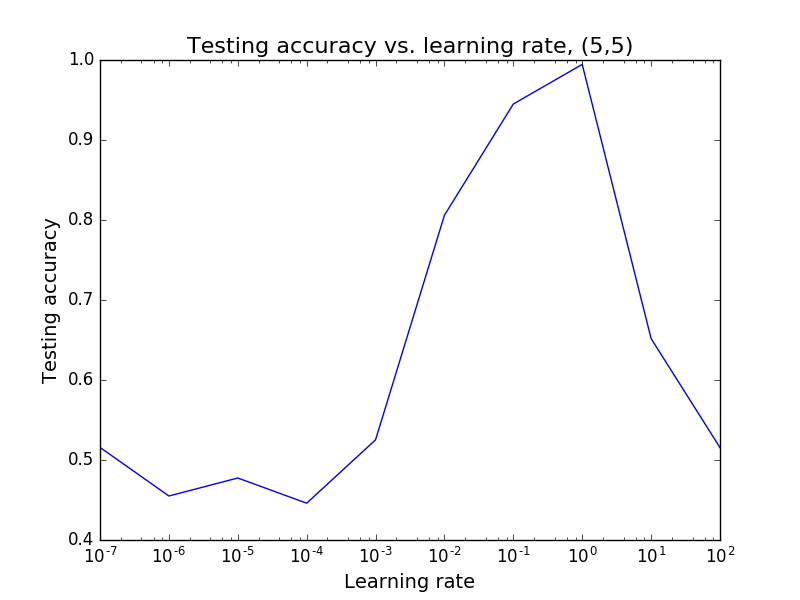
\includegraphics[width=1.2\linewidth]{code/P1/learning_rate_vs_accuracy,(5,5).png}
  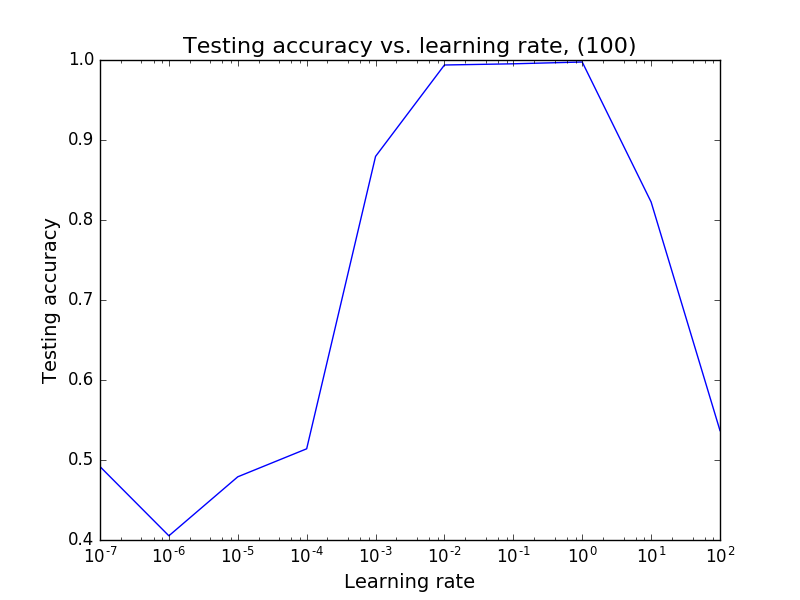
\includegraphics[width=1.2\linewidth]{code/P1/learning_rate_vs_accuracy,(100).png}
\end{multicols}
\caption{Learning rate vs. testing accuracy}
\end{figure}

Comparing these results with the accuracies from HW2, we see that the neural network performed significantly better than logistic regression with various types of regularization for non-linearly separable data. For linearly separable data, the accuracies were very comparable. Comparing these results with support vector machines, the neural network performed approximately as well as an SVM with a linear kernel for all the datasets with the exception of dataset 4, which displayed very poor performance. For SVMs with a radial basis kernel however, we were able to improve on the performance of a linear kernel SVM for dataset 4, and overall, the radial basis SVM displayed comparable, if not slightly improved performance, over neural nets. This comparative analysis is illustrated in Table 3, where the neural net accuracies are generated based on a neural net of one layer with 100 neurons per layer.

\begin{table}
  \begin{center}
    \begin{tabular}{ | c | c | c | c | c | }
      \hline
          & Logistic   & Linear SVM   & RBF SVM    & Neural net \\ \hline
      1   & 0.99       & 0.99         & 0.99       & 0.997        \\ \hline
      2   & 0.805      & 0.81         & 0.835      & 0.813        \\ \hline
      3   & 0.97       & 0.97         & 0.96       & 0.962        \\ \hline
      4   & 0.50       & 0.508        & 0.963      & 0.956        \\ \hline
    \end{tabular}
  \end{center}
  \caption{Testing accuracies of different algorithms}
\end{table}

\subsection{Multi-class classification}
We ran our neural network on the multi-class classification problem of identifying digits from the MNIST dataset. In our analysis, we used the same training, validation, and testing dataset sizes as suggested in HW2 for consistency. In this multi-class classification problem, we found that performance in identifying numbers was quite surprisingly low (at a little better than random chance). Nonetheless, we compared the testing accuracy against different numbers of neurons per layer, different numbers of hidden layers, and different learning rates for different neural network architectures.

Figure 2 illustrates the testing accuracy rate as a function of the number of neurons per layer in a one- and two-hidden layer neural network. It is interesting to note that in this case, accuracy increases as the number of neurons increases, which makes intuitive sense as an increased number of neurons can more effectively discover new features. Interestingly however, we do not observe a fall in the performance of the neural network at extremely large values of $n$, the number of neurons per layer (e.g. 1000), as one might expect could result due to overfitting. Here we simply see the performance of the network improve from a little better than random chance when $n=10$ to about 22\% when $n=1000$. The performance results for a one-layer neural network versus a two-layer neural network were found to be very comparable. Note that the accuracies calculated here are again an average of 20 runs of training.

\begin{figure}[width=\linewidth]
\centering
\begin{multicols}{2}
  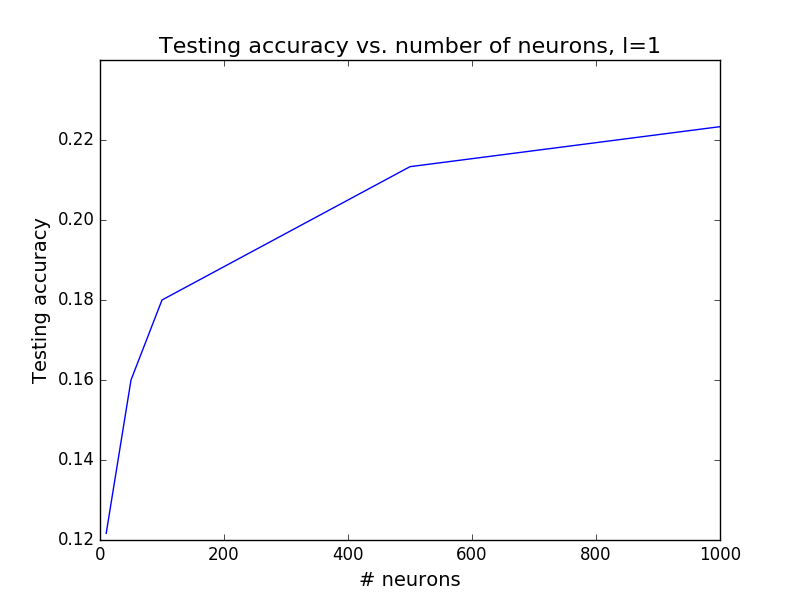
\includegraphics[width=1.2\linewidth]{code/P1/accuracy_vs_neurons,mnist.png}
  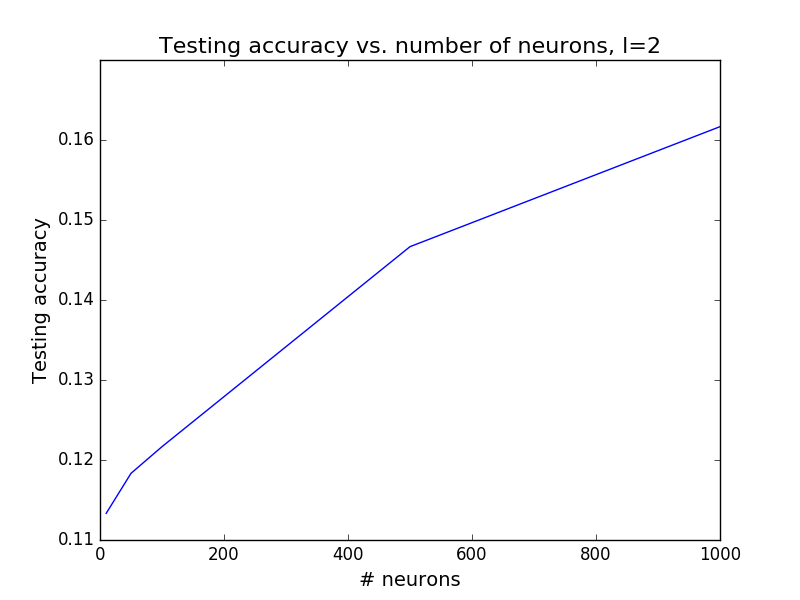
\includegraphics[width=1.2\linewidth]{code/P1/accuracy_vs_neurons,mnist,l2.png}
\end{multicols}
\caption{Number of neurons vs. testing accuracy}
\end{figure}

We additionally explored the testing accuracy as a function of the number of layers in the neural network. These results are presented in Figure 3, in which the neural network had 5 neurons and 100 neurons per hidden layer. Both sizes of neural networks had similar trends, in that performance generally peaked at around 2 or 3 hidden layers. Performance generally deteriorated for smaller or larger values of $l$, which is in support of our hypothesis that extremely complex neural nets might overfit to the training data and thus suffer during testing on unseen data samples. Furthermore, as is consistent with our hypothesis, we can see that peak performance for the neural network with five neurons per layer performed worse (at around 12\%) than the neural network with 100 neurons per layer (at around 18\%).

\begin{figure}[width=\linewidth]
\centering
\begin{multicols}{2}
  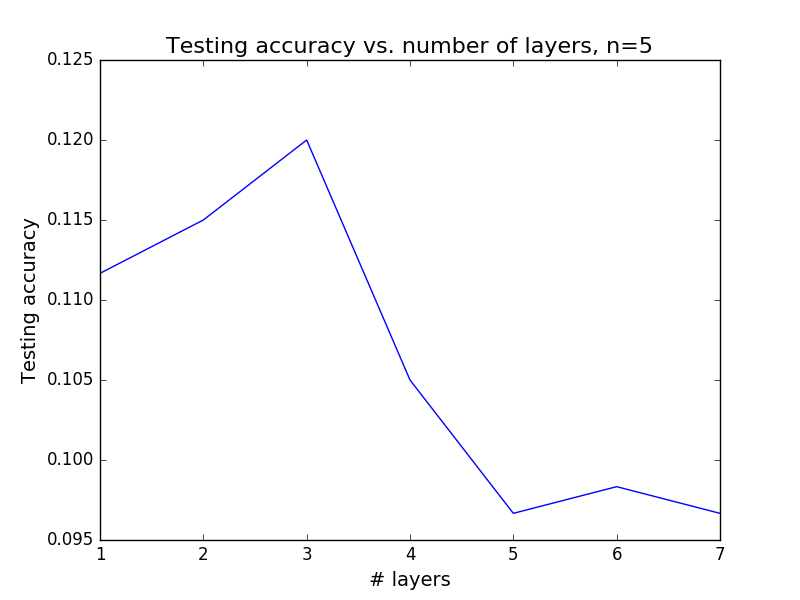
\includegraphics[width=1.2\linewidth]{code/P1/accuracy_vs_layers,mnist,n5.png}
  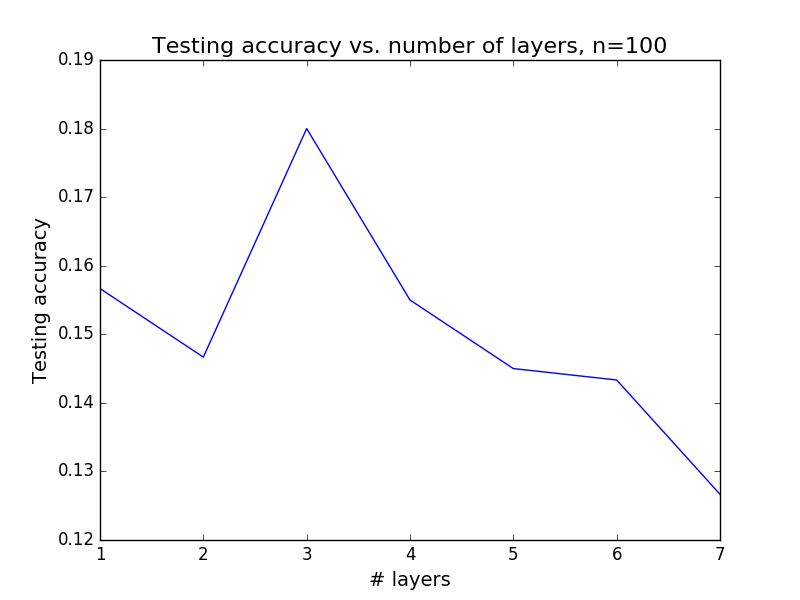
\includegraphics[width=1.2\linewidth]{code/P1/accuracy_vs_layers,mnist,n100.png}
\end{multicols}
\caption{Number of layers vs. testing accuracy}
\end{figure}

Figure 4 illustrates the relationship between the learning rate and the testing accuracy for neural networks of size $n=5,l=2$ and $n=100,l=1$. In this situation, we again found that there was an optimal learning rate, below and above which the performance of the neural network significantly suffered. Interestingly however, we found that the optimal learning rate for a neural network with $n=5, l=2$ was generally much smaller for the multi-class classification problem with MNIST ($\eta^*$ = 1\textsc{e}-5) than with the binary classification problem ($\eta^*$ = 1\textsc{e}-2). We did not observe this discrepancy in behavior comparing a neural network with $n=100, l=1$ in the multi-class classification problem versus in the binary classification problem ($\eta^*$ = 1\textsc{e}-2 for both).

\begin{figure}[width=\linewidth]
\centering
\begin{multicols}{2}
  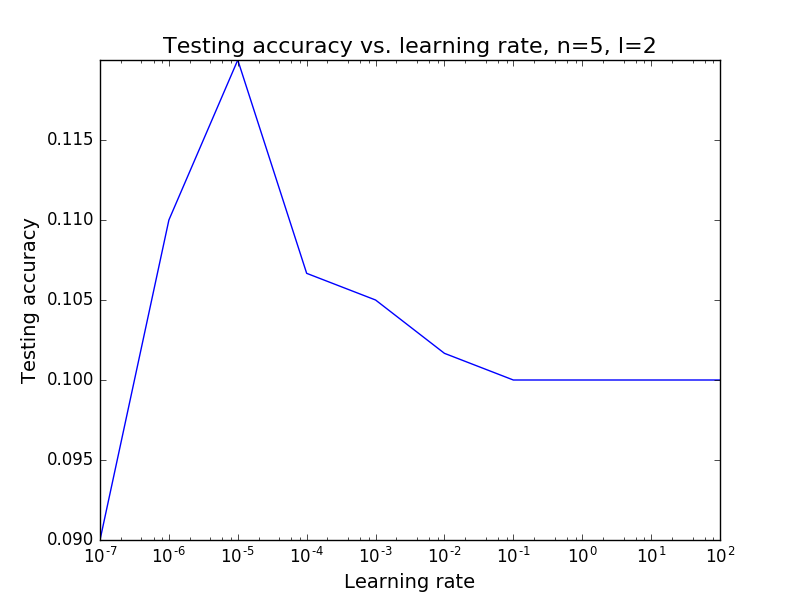
\includegraphics[width=1.2\linewidth]{code/P1/accuracy_vs_learning_rate,mnist,(5,5).png}
  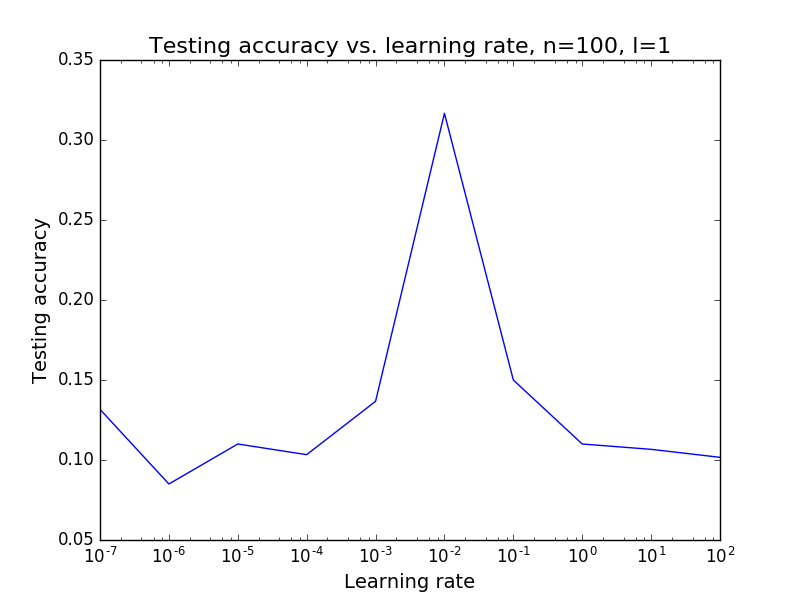
\includegraphics[width=1.2\linewidth]{code/P1/accuracy_vs_learning_rate,mnist,(100).png}
\end{multicols}
\caption{Learning rate vs. testing accuracy}
\end{figure}

Note that in this case, normalization of the data is especially important. This is because of the activation function we have chosen to use in each of the neurons of the hidden layers. More specifically, the ReLu activation function takes the maximum of 0 and $z$. For unnormalized data however, $z > 0$, and this activation function would not adequately fit the architecture of the neural network. Normalization is therefore essential in order to have the data input fit the architecture demanded by a neural network.

Overall we found that for the multi-class classification problem explored here, a neural network with 3 hidden layers and a large number of neurons per hidden layer (e.g. 1000) with an optimized learning rate performs best. We found that under this architecture, the optimal learning rate was $\eta^*=$1\textsc{E}-2 with a final testing performance of 39\% (Figure 4).

\begin{figure}[width=\linewidth]
\centering
  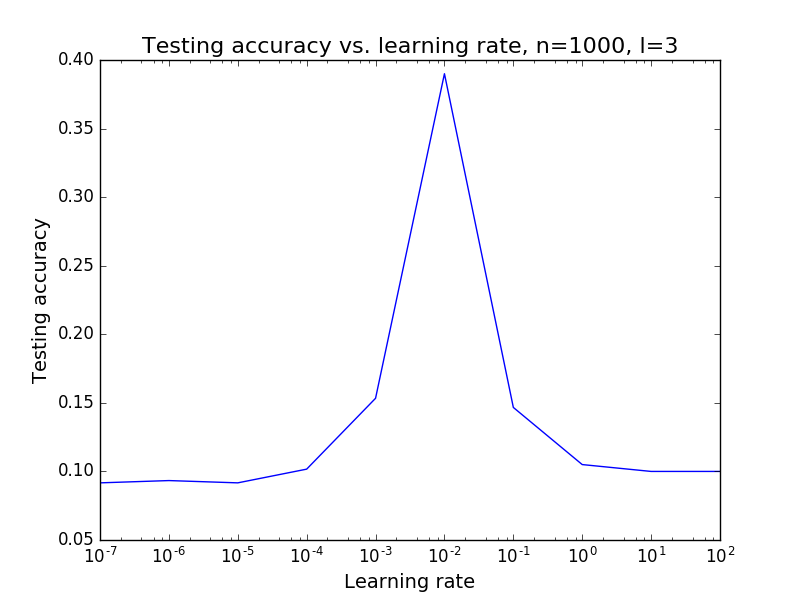
\includegraphics[width=0.8\linewidth]{code/P1/accuracy_vs_learning_rate,mnist,(1000,1000,1000).png}
\caption{Best neural network architecture}
\end{figure}


\section{Convolutional Neural Networks}
In this section, we explore the application of convolutional neural networks in performing image classification.

\subsection{Convolutional filter receptive field}
The dimensions of the receptive field for a node in $Z_2$ is $7 x 7$. With this in mind, we see that it is effective to build convolutional networks deeper in order to increase the receptive fields for subsequent nodes. This is effective because it allows the network to learn additional features that take into account larger and larger amounts of the original image's pixels.

\subsection{Run the Tensorflow conv net}
In the "define\_tensorflor\_graph" graph function we see that there could be a maximum of 6 layers and a minimum of 4 layers. Only 2 of the layers are convolutional. 2 other ones are regular hidden ones and the 2 optional ones are pooling layers. The relu activation function is used on the hidden nodes. The softmax loss function with cross entropy is being used to train the network. The loss is being minimized with gradient descent. When the convolutional network is run, we get a batch training accuracy of 100\% and a validation accuracy of 63.2\%. What this means is that the network is classifying extremely well on the training data, while not so well on the validation datasets, which points towards overfitting.

\subsection{Add pooling layers}
By adding pooling layers to our convolutional network, our results definitely changed. Specifically, we used a layer 1 pool filter size of 5, a layer 1 pool stride of 2, a layer 2 pool filter size of 2, and a layer 2 pool stride size of 2. After the 1500th step, this achieved a batch training accuracy of 100\% and a validation accuracy of 69\%. Interestingly enough, after the 1400th step, the training accuracy was 70\% and the validation accuracy was also 70\%. With these results it appears that max pooling marginally reduces the training accuracy while improving the validation accuracy. In a sense, it almost serves as a form of regularization that is able to prevent overfitting because now instead of the final layer processing information from all the original pixels the pooling allows clusters of pixels to be expressed as one value which enables better generalization.

\subsection{Regularize your network!}
\subsubsection{Dropout}
\subsubsection{Weight regularization}
\subsubsection{Data augmentation}
\subsubsection{Early stopping}

\subsection{Experiment with your architecture}

\subsection{Optimize your architecture}

\subsection{Test your final architecture on variations of the data}




\end{document}


% This document was modified from the file originally made available by
% Pat Langley and Andrea Danyluk for ICML-2K. This version was
% created by Lise Getoor and Tobias Scheffer, it was slightly modified
% from the 2010 version by Thorsten Joachims & Johannes Fuernkranz,
% slightly modified from the 2009 version by Kiri Wagstaff and
% Sam Roweis's 2008 version, which is slightly modified from
% Prasad Tadepalli's 2007 version which is a lightly
% changed version of the previous year's version by Andrew Moore,
% which was in turn edited from those of Kristian Kersting and
% Codrina Lauth. Alex Smola contributed to the algorithmic style files.
